\chapter{Introduction}
\label{ch:introduction}

\section{Motivation}
  Recent interest in advanced and next-generation nuclear power reactor designs 
  has encouraged further development of simulations for these reactors. A class 
  of advanced nuclear power reactors is Fast Reactor (FR), which operate with 
  predominantly high-energy (``fast'') neutrons in the fission reaction. Since 
  early development of FRs, such as the Experimental Breeder Reactor I (EBR-I) 
  in 1951 and Fermi 1 in 1956, there have been significant innovations in both 
  nuclear modeling and computational methods. As development of FRs is 
  revisited in the form of the Versatile Test Reactor (VTR) at Idaho National 
  Laboratory (INL), modern improvements in simulation can be used to simulate 
  FRs with modern best practices. These methods can easily be used for fast
  reactors with a variety of coolants including sodium, lead, or molten salt.

  Nuclear reactor simulations are inherently multi-physics simulations. For
  example, neutron reaction probabilities are described by cross-sections.
  Neutron cross-sections are dependent on material temperatures and densities,
  both of which vary over the operating range of a nuclear power reactor. As
  reactor power changes, material temperatures and densities change, therefore
  cross-sections change and affect the reactor power. The multi-physics nature
  of the reactor necessitate a simulation of the power distribution within the
  reactor as well as all physical effects which will be modeled. 
  
  In this thesis, models for simulating FRs will be developed and demonstrated. 
  Reactor power distribution will be modeled according to the multigroup neutron
  diffusion equation as solved by the Finite Element Method (FEM) based on
  unstructured meshes in hexagonal/triangular geometry. The multigroup neutron
  diffusion solution code is verified through both benchmark and analytic
  solutions. Multi-physics effects are modeled including heat transfer and 
  thermal expansion. Thermal hydraulic effects are modeled as axial heat 
  convection and radial heat conduction. Thermal expansion is modeled using 
  simplified linear expansion models.

  By employing a modern solution method to the neutron diffusion
  equation in the form of the FEM, the simulation can take advantage of 
  developments in numerical methods including the solution of linear systems. 
  Additionally, the simulation allows for the incorporation of generalized 
  multi-physics effects whereas current state-of-the-art simulations require 
  data processing and manual iteration to simulate multi-physics effects. The 
  final simulation is designed to simulate an operating FR and estimate 
  feedback coefficients.

\section{Geometry Description}
  \label{sec:geometry_description}
  Fast reactor spectra operate in a regime with smaller neutron cross-sections.
  To compensate for this fact, FRs are typically designed with hexagonal,
  triangularly pitched, fuel assemblies to maximize the fuel packing and
  increase the fuel density. An example of an FR with hexagonal geometry
  is shown in \fref{fig:reactor_materials}.
  This geometry is used to describe material properties in the form of 
  cross-sections as well as to describe coolant flow geometries. Dimensions of 
  assemblies are measured at room temperature and will later be expanded 
  according to the thermal expansion model in \chref{ch:thermalExpansion}.
  
  \begin{figure}
    \centering
    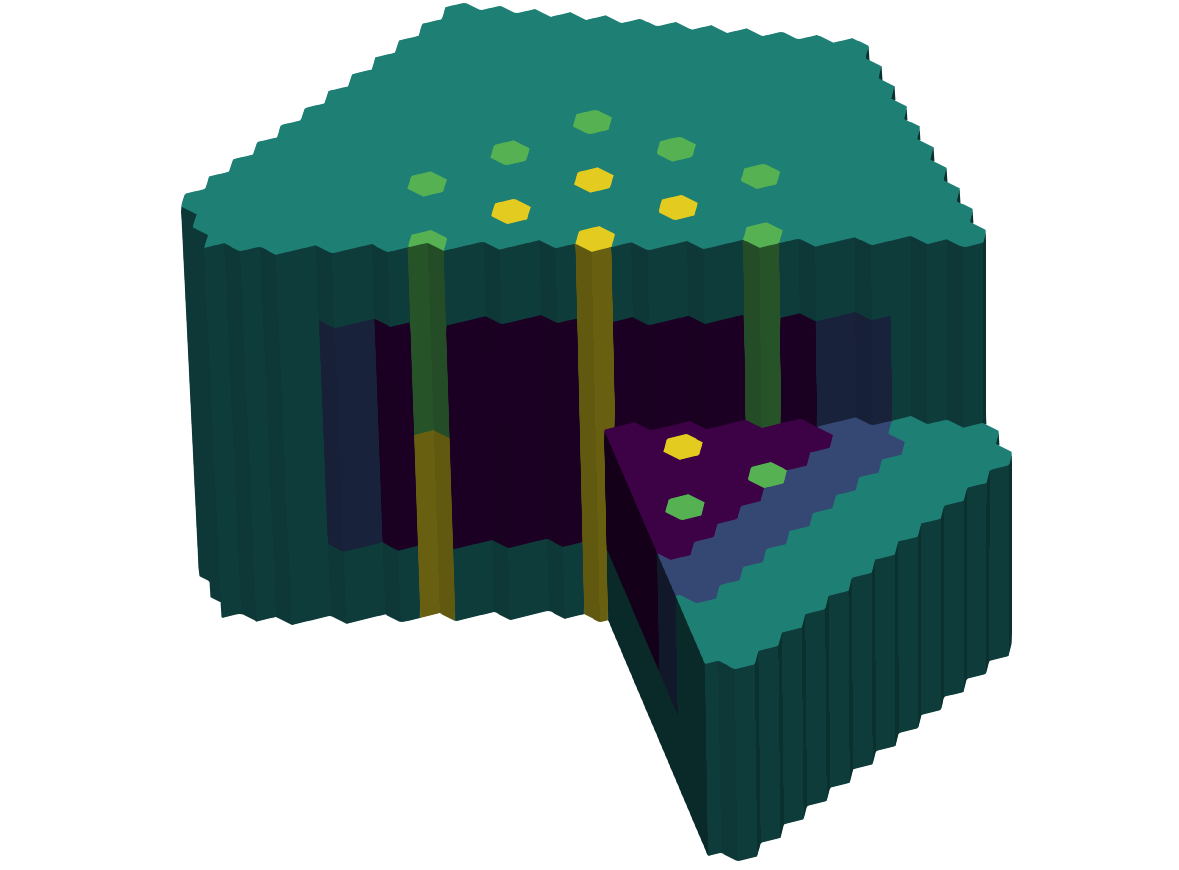
\includegraphics[width=\textwidth]{reactor_materials}
    \caption{Example of Fast Reactor Materials based on MONJU.}
    \label{fig:reactor_materials}
  \end{figure}

  \begin{figure}
    \centering
    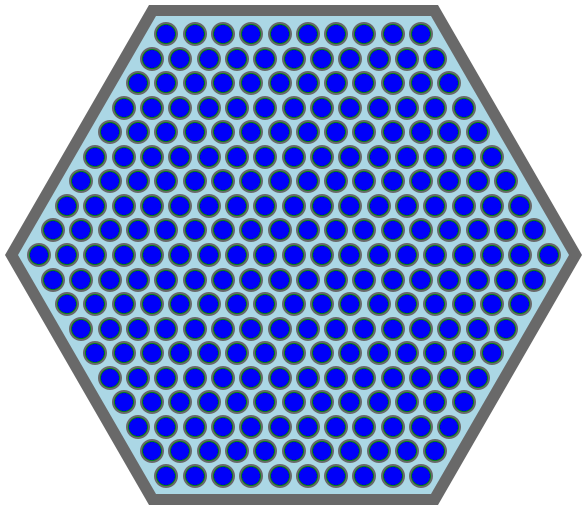
\includegraphics[width=0.5\textwidth]{prism_hex}
    \caption{Example of Fast Reactor Fuel Assembly Cross-section.}
    \label{fig:prism_hex}
  \end{figure}

  A cross-sectional representation of a hexagonal assembly, is shown in 
  \fref{fig:prism_hex}. 
  Note the individual material rods are cylindrical and are arranged
  into a hexagonal assembly. The basic geometry is a fuel material within
  stainless steel cladding. The gap between the fuel and cladding is filled by
  sodium bond to improve thermal conductivity across the gap. The rod is
  wrapped by a steel wire to ensure separation between rods that will allow for
  coolant flow. The wire wrap also serves to encourage the mixture of coolant
  within the assembly. (Note: wire wrap is omitted from \fref{fig:prism_hex}.) 
  Many rods are then assembled into an assembly and surrounded by a hexagonal 
  can made of steel. This can aids in structural stability and prohibits 
  cross-flow between assemblies. 

  The dimensions within a single rod are shown in \fref{fig:pin_model} and the
  dimensions within a hexagonal assembly can are shown in \fref{fig:hex_can}. In
  \fref{fig:hex_can}, $T\!h_{Can}$ is the thickness of the assembly can,
  $F\!2\!F$ is the flat-to-flat measurement of the outside of the hexagonal can,
  and \textit{Pitch} is the distance between the center of two rods.
  Using the geometry described in 
  these figures, the material cross-sectional areas are calculated according to 
  the given formulae where $N_{rod}$ is the number of rods in the assembly.
  \begin{align}
    \label{eq:afrac_first}
    A_{total} &= \frac{\sqrt{3}}{2} F\!2\!F^2 \\
    A_{can} &= A_{total} - 
      \frac{\sqrt{3}}{2} \left(  F\!2\!F - 2 \, T\!h_{Can} \right) \\
    A_{wrap} &= N_{rod} \frac{\pi}{4} D_{wrap}^2 \\
    A_{clad} &= N_{rod} \pi (R_C^2 - R_B^2) \\
    A_{bond} &= N_{rod} \pi (R_B^2 - R_F^2) \\
    A_{fuel} &= N_{rod} \pi R_F^2 \\
    \label{eq:afrac_last}
    A_{cool} &= A_{total} - A_{can} - A_{wrap} - A_{clad} - A_{bond} - A_{fuel}
  \end{align}
  Calculating the areas as above allows for calculation of cross-sectional area
  fractions. Assuming constant dimensions in the axial
  direction, these area fractions are equivalent to volume fractions and are
  useful for neutron cross-section calculations. Additionally, these formulae
  allow for thermal expansion as the liquid sodium in the bond and
  the liquid coolant are allowed to vary to allow for the expansion of other 
  materials.

  \begin{figure}
    \centering
    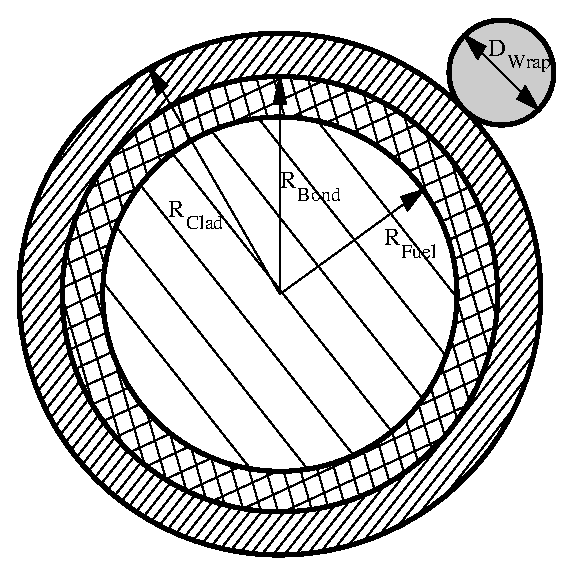
\includegraphics[width=0.5\textwidth]{pin_model}
    \caption{Dimensions of Thermal Hydraulic Rod Model.}
    \label{fig:pin_model}
  \end{figure}

  \begin{figure}
    \centering
    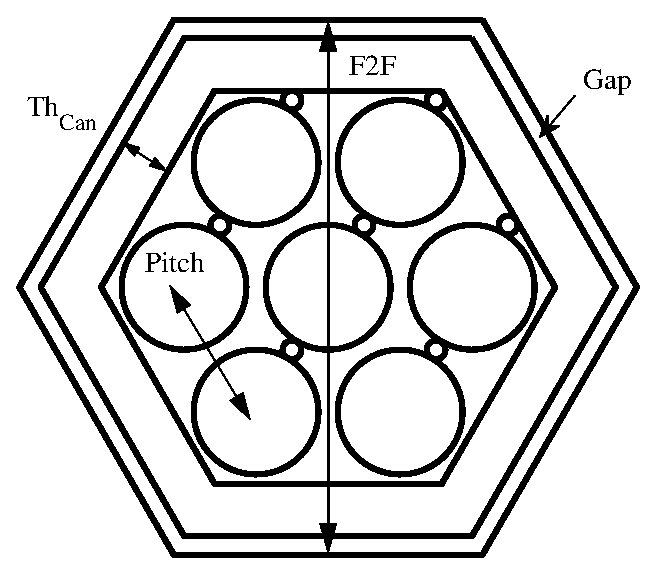
\includegraphics[width=0.5\textwidth]{hex_can}
    \caption{Dimensions of Hexagonal Can.}
    \label{fig:hex_can}
  \end{figure}

\section{Cross-Section Treatment}
  \label{sec:cross_section_treatment}
  Reactor materials are ``smeared'' into homogeneous regions. This assumption is 
  common to fast reactors because of the relatively large neutron 
  mean-free-paths compared to the scale of material dimensions. 
  The natural choice for these homogenized regions are the hexagonal
  assemblies themselves. Materials are permitted to be heterogeneous axially but
  For this simulation, four distinct regions are modeled representing fuel, 
  bond, coolant, and steel. Steel material includes cladding, wire wrap, and 
  assembly can. 

  For benchmark and analytic problems material, cross-sections are given as
  constants. Realistic reactor simulations require
  cross-sections generated from preliminary calculations. In this
  work, multigroup microscopic cross-sections are generated using the computer
  program \mcc \cite{mcc}.
  The cross-section generator uses 2,082 fine energy groups to collapse down
  to an arbitrary number of energy-groups. For this simulation, the
  recommended and default 33-group energy structure is used. \mcc 
  solves for the cross-sections in an infinite homogeneous medium and isotopic 
  number densities are calculated and input by the user.
  Cross-sections for each assembly type are generated separately to accurately
  simulate the neutron energy spectrum within the assembly. The neutron fission  
  spectrum for fissile media is generated by the media's fission spectrum. 
  Non-fissile homogenized mixtures, such as control assemblies or reflector
  assemblies, use the default \isotope[238]{U} fission spectrum. 

  To capture the effect of Doppler broadening, cross-section libraries are
  generated for several different region temperatures. These libraries are
  then used during the simulation to calculate on-the-fly cross-sections as a
  function of region temperatures.
  The fuel, clad, and coolant temperatures can be calculated with a thermal
  hydraulic model (see \chref{ch:thermalHydraulics}), these relationships are 
  functions of reactor power and coolant mass flow rate. These parameters are
  not known before the simulation for a general reactor. Instead, a simplified
  temperature relationship is used to generate the cross-section libraries.

  In each cross-section library, the coolant is maintained at some nominal
  temperature. For this work, that temperature is $400 \units{K}$. Maintaining 
  the coolant temperature as constant in this manner is acceptable because the 
  dominant effect of temperature on the macroscopic cross-sections in the 
  coolant is the density change of the fluid, not the Doppler effect. With
  constant coolant temperature, the fuel temperature is then varied over some 
  range. In this work, libraries are generated for average fuel temperatures
  of $400 \units{K}$, $600 \units{K}$, $900 \units{K}$, and $1200 \units{K}$.
  At each fuel temperature, the clad temperature is related as 
  \begin{equation}
    T_{clad} = \max \left\{ w \, T_{fuel}, T_{cool} \right\}
  \end{equation}
  % note: weight for T_{cool} should be 0.63 if perturbed coolant is desired
  where $w$ is a weighting factor, $T_{fuel}$ is the chosen fuel temperature
  for the library, and $T_{cool}$ is the chosen coolant temperature for the
  library. A weighting of $w=0.7$ was selected based on analysis of the ratio
  $T_{clad}/T_{fuel}$ for a representative high power channel
  within an example reactor simulation.  Temperature in non-fissile assemblies 
  is set to $T_{cool}$ during the collapse as there is no heat generation 
  modeled in these regions.

  \begin{table}
    \caption{Temperatures Selected for Cross-section Libraries.}
    \label{tab:xstemps}
    \begin{center}
      \begin{tabular}{lll}
        \toprule
        $T_{cool} \units{K}$ & $T_{clad} \units{K}$ & $T_{fuel} \units{K}$ \\
        \midrule
        628.15 & 628.15 & 628.15  \\
        628.90 & 681.90 & 717.90  \\
        708.65 & 757.50 & 807.15  \\
        ??? & ??? & ??? \\
        \bottomrule
      \end{tabular}
    \end{center}
  \end{table}

  Ultimately, the microscopic cross-sections are accumulated in four separate 
  libraries at temperatures given in \tref{tab:xstemps}. Then, these libraries 
  are used to calculate on-the-fly cross-sections during the simulation using a
  temperature interpolation method.
  For each region, average macroscopic cross
  sections are calculated by homogenizing the microscopic cross-section and with 
  number densities $N_{i,j}$ for isotope ${j=1,2,\ldots,N_{iso}}$ in region
  ${i=1,2,\ldots,N_{reg}}$.  For the $x$ reaction type, the 
  macroscopic cross-section in each region is defined as
  \begin{equation}
    \Sigma_{x,g}^r = \frac{\sum_{i=1}^{N_{reg}} \sum_{j=1}^{N_{iso}} V_i N_{j} 
      \sigma_{x,g,i}} {\sum_{i=1}^{N_{reg}}V_i}
  \end{equation}
  where the superscript $r$ corresponds to the region. Assuming cross sectional
  areas within the assembly are constant within a given axial elevation, area
  fractions can be treated as volume fractions. These area fractions are
  calculated according to the area formulae from \eref{eq:afrac_first} through
  \eref{eq:afrac_last}. Finally, the homogenized transport cross section is used 
  to calculate the diffusion coefficient.
  \begin{equation}
    D_g^r = \frac{1}{3 \Sigma_{tr,g}^r}
  \end{equation}

\section{Thesis Organization}
  In \chref{ch:neutronDiffusion}, the derivation of the FEM solution to the
  multigroup neutron diffusion equation is
  presented for triangular and wedge elements. The resulting eigenvalue problem
  is solved using the Power Method. Results from the diffusion solution are
  verified in two-dimension and three-dimension problems with both analytic and
  benchmark solutions. These verification problems for the neutron diffusion
  equation are presented in \chref{ch:diffusionResults}.

  \chref{ch:thermalHydraulics} presents the formulation of axial heat convection
  and radial heat conduction models for a typical FR. These models are used to
  calculate material temperatures and update cross-sections for the simulation.
  Results of the numerical model is compared to analytical models and example
  system temperatures are shown.

  The materials are expanded according to thermal expansion behavior as
  described in \chref{ch:thermalExpansion}. 
  
  All of these models allows for the realistic
  simulation of an FR and results of the simulation of a model FR are presented
  in \chref{ch:coupledResults}.
 
  Finally, \chref{ch:conclusions} presents a 
  summary and the conclusions of this research. Additionally, recommendations 
  for further research are included.

